 %==================================================================================================
%   LUKES THESIS TEMPLATE 1.2
%   -------------------------
%   This template is based upon the offcial IMM PhD Thesis template, it is enhanced with a number
%   of new features and a number of errors have fixed. This template is intended to be complied to
%   PDF using PDFLATEX and is tested using the MiKTeX 2.9 LaTeX distribution.
%   It is based on the official DTU-IMM Thesis template by Finn Kuno Christensen in 2009.
%   Small bugfixes by Kasper Laursen in 2012 and 2013.
%   Small updates by Finn Kuno Christensen/Henning Christiansen in 2015.
%   -------------------------
%   Last Updated: 2015-01-08
%==================================================================================================
%
%==================================================================================================
% DOCUMENT SETUP
%==================================================================================================
\documentclass[10pt,twoside]{book}                  %Official DTU-IMM Thesis document setup
%
%Set to 'print' for printed version, use 'net' for online version
\def\thesisversion{net}
%
%==================================================================================================
% PACKAGES
%==================================================================================================
\usepackage{LukeThesis}                             %Import Thesis base style
\usepackage{pdfpages}
\usepackage{mwe,tikz}
\usepackage{tocloft}
\usepackage{xcolor}
\usepackage{rotating}
\usepackage{siunitx}
\sisetup{inter-unit-product =\ensuremath{{}\cdot{}}}
\newcommand{\siunit}[1]{\ \ \ [\SI{}{#1}]}
\newcommand{\siunitnospace}[1]{[\SI{}{#1}]}
\setlength{\cftchapnumwidth}{2.5em}
%\newcommand{\fixme}[1] { \textcolor{red}{\textbf{FIXME: } #1}}
\newcommand{\fixme}[1] {}
\usetikzlibrary{positioning}
%input{PhDMacros}                                   %Thesis specific macros
%
%==================================================================================================
% THESIS PROPERTIES (Modifiy these fields with your details)
%==================================================================================================
\def\thesisauthor{Alessandro Dal Corso}                     %Author
\def\thesistitle{Hybrid techniques for interactive photorealistic rendering}               %Title
\def\thesishandin{31-March}                       %Submission date (Day-Month}
\def\thesisdegree{PhD}                              %Degree ('B.Eng', 'B.Sc.', 'M.Sc.' or 'PhD')
\def\thesisyear{2017}                               %Submission year
\def\thesisnumber{????}                             %DTU-IMM Serial number (do not include year)
\def\thesisISSN{0000-0000}                          %ISSN number
\def\thesiskeywords{rendering, materials}  %PDF keywords
\derivethesisprops                                  %Derive dependent properties
%
%==================================================================================================
% SECTION NUMBERING SETUP
%==================================================================================================
\setcounter{tocdepth}{2}                            %2 adds sections up to subsections
\setcounter{secnumdepth}{3}                         %Subsubsections get a number when this is 3
%
%==================================================================================================
% THESIS STRUCTURE  (Modifiy to include more chapters etc)
%==================================================================================================
\begin{document}
%------------------------
%Pre-frontmatter material
%------------------------
\prefrontmatter
%--------------------
%Frontmatter material
%--------------------
\frontmatter
\pagenumbering{roman}                               %Set frontmatter numbering style
\chapter{Summary}

Interactive rendering applications are becoming more and more prominent in everyday life. In many fields, including manufacturing, product design and entertainment, photorealistic rendering is becoming more and more prominent, in order to correctly predict appearance of complex materials. So, in many interactive applications, there is a need for fast interactive techniques that achieve based on physically based principles. 

In this thesis, we address the challenge of proposing new photorealistic interactive rendering techniques, that leverage the parallel power of graphics processing unit (GPUs) in order to effectively create renderings based on physical principles. These techniques propose effective caching and filtering schemes in order to efficiently reuse data, both spatially and temporally.     
 
This thesis offers insight into different areas of computer graphics, including scene reconstruction, material parameter estimation, efficient data structures and physically based rendering models. In addition, we explore the different compromises and trade-offs that are necessary to achieve accurate photorealistic renderings. More specifically, we contribute with two innovative techniques: the first relates to fast rendering of translucent materials and includes directional effects of subsurface scattering into consideration. The second technique contributes with a fast reprojection scheme to improve temporal stability in interactive ray tracing, that can be easily applied on top of existing rendering algorithms. On top of these, we propose an innovative validation pipeline to compare renderings with actual images, with the final purpose of validating existing rendering and reconstruction techniques against a picture of the real world. 

With these contributions, this thesis proves how it is possible to use effective caching schemes to effectively improve existing techniques to handle more complex optical effects, maintaining the time constraints of interactive rendering environments.                                   %English summary of Thesis
\markboth{}{}                                       %Set headings (left)(right)
\chapter{Summary (Danish)}
\begin{otherlanguage}{danish}

\end{otherlanguage}                      
             %Danish summary of Thesis
\markboth{}{}                                       %Set headings (left)(right)
\chapter{Preface}

The work from this Ph.D. thesis was carried under the Section for Image Analysis and Computer Graphics, at the Department for Applied Mathematics and Computer Science (DTU Compute) at the Technical University of Denmark (DTU). This thesis was prepared in fulfillment of the requirements to obtain a doctor of philosophy (Ph.D.) in computer science. The work presented was funded on a DTU Compute internal scholarship. 

This thesis deals with the topic of bringing techniques from photorealistic offline rendering into the interactive and real time domain. To achieve this goal, a set of publications was produced over the course of the studies. The publications are summarized at page~\pageref{sec:contributionlist}. Relevant  publications for this thesis are available for the sake of the reader in Appendices~\ref{sec:firstcontribution}-\ref{sec:mertensnote}. From these, a total of five peer reviewed publications have been included in this thesis (\ref{sec:firstcontribution}-\ref{sec:lastcontribution}), while two (X-XI) have been left out as not relevant to the overall thesis topic. Moreover, during the course of the Ph.D. some notes were produced. These notes are reported as non peer reviewed material and attached in Appendices~\ref{sec:jensennote}-\ref{sec:mertensnote}. 

The work has been carried under the main supervision of Associate Professor Jeppe Eliot Revall Frisvad, with the co-supervision of Associate Professor Andreas B\ae rentzen. The research activities have mostly been conducted at DTU, with the exception of two external research stay periods. The first research stay was an internship at NVIDIA Corporation, under managers Aaron Lefohn and David Luebke, in the real time rendering research team based in Redmond, Washington, USA. The second external research stay was under the supervision of Professor Toshiya Hachisuka, Department of Creative Informatics, The University of Tokyo.

%==================================================================================================
% SIGNATURE AREA
%==================================================================================================
\vspace{20mm}
\begin{center}
    \hspace{20mm} Lyngby, \thesishandin-\thesisyear
    \vspace{5mm}
    \newline
  %Update signature image file in line below
    \includegraphics[scale=0.5]{figures/signature}
\end{center}
\begin{flushright}
    \thesisauthor
\end{flushright}
% % % EOF % % %                                     %Preface
\markboth{}{}                                       %Set headings (left)(right)
\chapter{Acknowledgements}

First and foremost, I would like to thank my supervisors Jeppe Revall Frisvad and Andreas B\ae rentzen. In particular, I would like to thank Jeppe for the support during the PhD, the deep technical discussions and a push to strive for perfection. I would like to thank Andreas for the deep and interesting discussion on how to push my work towards more and more challenging directions. I would also like to thank my managers and mentors during my internship at the real-time rendering research group in NVIDIA: Craig Kolb, Marco Salvi, Aaron Lefohn and David Luebke, for sharing some of their deep knowledge about graphics. Finally, I would like to thank Toshiya Hachisuka and its group for hosting me at Tokyo University, for the their hospitality and the interesting discussions.

I would like to thank DTU Compute for financing my scholarship and giving me the opportunity to pursue a PhD in the realm of computer graphics.

A great thank you of course goes to my colleagues, collaborators, and office mates at the section for Image Analysis and Computer Graphics. Thank you for the continuous support, the coffee calls, and the general silliness that makes everyday a fun day to come to the office. It has been a great pleasure to be part of this section, sharing thoughts and ideas, and having interesting discussion over a coffee.

Last but not least, I would like to thank my loving family and friends. Without your continuous support and help, I would not have been able to complete this endeavor.                             %Acknowledgements
\markboth{}{}                                       %Set headings (left)(right)
%------------------
% Table of contents
%------------------
\newpage\mbox{}\newpage
\chaptermark{Contents}
\pdfbookmark{\contentsname}{toc}
\renewcommand{\sectionmark}[1]{\markright{#1}}
\sectionmark{Contents}
\addtolength{\parskip}{-\baselineskip}
\tableofcontents
\addtolength{\parskip}{\baselineskip}
\renewcommand{\sectionmark}[1]{\markright{\thesection\ #1}}
%-------------
% Main content
%-------------
\chapter*{List of contributions}
\label{sec:contributionlist}
\section*{Peer rewiewed}
\begin{itemize}
\item \textbf{Alessandro Dal Corso}, Jeppe Revall Frisvad, Jesper Mosegaard, and J. Andreas Bærentzen. Interactive directional subsurface scattering and transport of emergent light. \textit{The Visual Computer}, 33(3):371–383, Mar 2017.~\cite{dalcorso17dirsss}
\item Jonathan Dyssel Stets, \textbf{Alessandro Dal Corso}, Jannik Boll Nielsen, Rasmus Ahrenkiel Lyngby, Sebastian Hoppe Nesgaard Jensen, Jakob Wilm, Mads Brix Doest, Carsten Gundlach, Eythor Runar Eiriksson, Knut Conradsen, Anders Bjorholm Dahl, Jakob Andreas Bærentzen, Jeppe Revall Frisvad, and Henrik Aanæs. Scene reassembly after multimodal digitization and pipeline evaluation using photorealistic rendering. \textit{Applied Optics}, 56(27):7679–7690, Sep 2017.~\cite{stets17}
\item \textbf{Alessandro Dal Corso}, Marco Salvi, Craig Kolb, Jeppe Revall Frisvad, Aaron Lefohn, and David Luebke. Interactive stable ray tracing. In \textit{Proceedings of High Performance Graphics}, HPG ’17, pages 1:1–1:10, New York, NY, USA, 2017. ACM. \cite{dalcorso17hpg}
\item \textbf{Alessandro Dal Corso}, Jonathan Dyssel Stets, Andrea Luongo, Jannik Boll Nielsen, Jeppe Revall Frisvad, and Henrik Aanæs. Virtual reality inspection and painting with measured brdfs. In \textit{SIGGRAPH Asia 2017 VR Showcase}, SA ’17, pages 15:1–15:2, New York, NY, USA, 2017. ACM.~\cite{dalcorso17vr}
\item \textbf{Alessandro Dal Corso}, Jeppe Revall Frisvad, Thomas Kim Kjeldsen, and Jakob Andreas Bærentzen. Interactive Appearance Prediction for Cloudy Beverages. In Reinhard Klein and Holly Rushmeier, editors, \textit{Workshop on Material Appearance Modeling}. The Eurographics Association, 2016.~\cite{dalcorsomam16}
\end{itemize}

\section*{Non included}
\begin{itemize}
\item Henrik Aanæs, Knut Conradsen, \textbf{Alessandro Dal Corso}, Anders Bjorholm Dahl, Alessio Del Bue, Mads Emil Brix Doest, Jeppe Revall Frisvad, Sebastian Hoppe Nesgaard Jensen, Jannik Boll Nielsen, Jonathan Dyssel Stets, et al. Our 3d vision datasets in the making. In CVPR Workshop: The Future of Datasets in Vision 2015, 2015.~\cite{aanaes2015our}
\item \textbf{Alessandro Dal Corso}, Mikkel Olsen, Kasper Hornbak Steenstrup, Jakob Wilm, Sebastian Jensen, Rasmus Reinhold Paulsen, Eythor Eiríksson, Jannik Boll Nielsen, Jeppe Revall Frisvad, Gudmundur Einarsson, and Hans Martin Kjer. Virtualtable: A projection augmented reality game. In \textit{SIGGRAPH Asia 2015 Posters}, SA ’15, pages 40:1–40:1, New York, NY, USA, 2015. ACM.~\cite{dalcorsosig15}
\end{itemize}

\section*{Unpublished material}
\begin{itemize}
\item \textbf{Alessandro Dal Corso, Jeppe Revall Frisvad, Thomas Kim Kjeldsen}. \textit{Derivation of standard and directional dipole quantities.} Unpublished note. Text in Appendix~\ref{sec:jensennote}.
\item \textbf{Alessandro Dal Corso, Jeppe Revall Frisvad}. \textit{On measuring BSSRDFs.} Unpublished note. Text in Appendix~\ref{sec:bssrdfnote}.
\item \textbf{Alessandro Dal Corso, Jeppe Revall Frisvad}. \textit{Point cloud method for rendering BSSRDFs.} Unpublished note. Text in Appendix~\ref{sec:pointcloudnote}.
\item \textbf{Alessandro Dal Corso}. \textit{Note on efficient color calibration}. Unpublished note. Text in Appendix~\ref{sec:colornote}.
\item \textbf{Alessandro Dal Corso}. \textit{Note on BSSRDF importance sampling from the camera, derivation from Mertens et al.}. Unpublished note. Text in Appendix~\ref{sec:mertensnote}.
\end{itemize}



\mainmatter
%Chapter 1
\chapter{Introduction}

\section{Scope}

\section{Motivation}

\section{Outcome}

\section{Outline}                                  %Chapter 1
\chapter{Background}
\begin{itemize}
\item Introduction of relevant theory behind the thesis
\item In photorealistic, introduction to most relevant quantities, namely radiometric quantities, brdfs and bssrdfs. Scattering and non scattering media.
\item Offline and real time techniques. GPUs. 
\item ray tracign and rasterization. bleeding between the two.
\end{itemize}

\section{Photorealistic rendering}

\begin{itemize}
\item Radiometric quantities. Flux radiance irradiance intensity
\item Reflectance functions
\item Scattering, RTE
\item Absorption, Beer's law
\item BRDF
\item BSSRDF
\item Empirical models (BRDF, BSSRDF)
\end{itemize}

\subsection{Rendering techniques}
\fixme{Discuss with Jeppe whether to move in Related work?}
\begin{itemize}
\item The rendering equation
\item Path tracing
\item Rendering with reflectance functions
\end{itemize}

\section{Real time rendering} 
\begin{itemize}
\item Modern GPUs
\item Fast rendering techniques
\item Raytracing 
\item Rasterization
\end{itemize}
                                                                                                                                                                                                                                                                           %Chapter 1
\chapter{Related work}
%
\label{sec:related}
%
In this section, we present some related work on the overall topic of the thesis, namely physically based techniques brought into the interactive domain. We will make use of the background theory we presented in Chapter~\ref{sec:background}, to better discuss our contributions in Chapter~\ref{sec:contributions}. This section is not meant to be a complete survey on such techniques, but we will point to the most important contributions, referring to a number of individual papers and surveys for a more complete overview. In particular, we point out the survey by Ritschel et al.~\cite{Ritschel2012} for a good overview on various interactive techniques for global illumination. We also refer to the related work of the individual contributions in the Appendices for more detailed literature in the context of the individual contributions. 
%
As we mention in Chapter~\ref{sec:intro}, interactive rendering requires a compromise between accuracy and speed. There are various examples in literature on the compromises that are needed to hit this trade-off. Since the rendering time constraints are usually set, compromises are usually done in physical accuracy. We will start by discussing some of the assumptions that are usually employed in interactive rendering environments. 
%
\section{Typical approximations in physically based rendering}

One of the natural approaches into achieving interactive photorealistic rendering is making some assumptions about our physical simulation. In principle, we can describe any light interaction by running a brute-force simulation of all the photons interacting with the particles of the material, then measuring the number of photons arriving at a set light sensor. Of course, running this sort of computation, even for extremely simple scenes, in reasonable times is not possible. In general, Monte Carlo path tracing~\cite{Kajiya1986} with extension to scattering media~\cite{Rushmeier1988} is considered a ground truth technique to generate reference images. Path tracing is an unbiased technique (i.e. converges always to the correct solution), but it gives extremely noisy results, especially for particular configurations of light and camera positions. To solve this problem, the offline rendering community proposed various improvements to reduce variance in path tracing, such as importance sampling~\cite{Kirk1991},multiple importance sampling~\cite{Veach1995}, Metropolis sampling~\cite{Veach1995}, Bidirectional path tracing~\cite{Veach1997}, manifold exploration~\cite{Jakob2012}, gradient-domain path tracing~\cite{Kettunen2015}, etc. The book by Pharr et al.~\cite{Pharr2017} gives a good overview of different path tracing techniques. We described one of these importance sampling techniques in Section~\ref{sec:volumept}, where we derived a formulation for interactive volume path tracing.

So when we need interactivity, different approximations can be used. Once we know the underlying physical process, different choices can be made on a per material basis. For example, in the case of most metals, the scattering of light is fairly limited around the point of incidence, so the BRDF approximation described in Section~\ref{sec:brdfsec} can be used. In the case of scattering materials, we can use the analytical BSSRDFs described in Section~\ref{sec:analyticalbssrdf} instead of a fully path traced simulation. Depending on the directionality of the scattering effects, different models can be used, at the price of increased rendering times. In applications such as games or virtual reality, often it is not even possible to use BSSRDF models, using an approximate BRDF instead. This gives acceptable results, but since scattering effects are important, this result in a "waxy" effect. This is particular noticeable in the case of skin. 

Another approach, instead of simplifying the physical model, real measured data can be used instead. This is the approach for example used by the discretized BRDF described in Section~\ref{sec:empiricalbrdf}. The drawback of measured materials is that they often require large storage spaces. This is often a problem, since most rendering pipelines are memory-bound. Discretized models often have discretization issues, and require particular care in deciding a proper storage space, such as the Runsinkewitz parameterization for measured BRDF. Finally, measured data are limited to the setup used to generate them. In the empirical BSSRDF by Donner et al.~\cite{Donner2009} the BSSRDF is simulated as a Monte Carlo path traced simulation. Many assumptions are required to simulate the BSSRDF in reasonable times, reducing the fourteen dimensions of the BSSRDF to a more tractable five.  

So far we have discussed material simplification. In general, the light hierarchy of a scene can also be object of simplification. Generically, a light is an object like any other in the scene, but that also emits light in the visible spectrum. In a path tracing context, lights are easily handled by the $L_e$ term in Equation~\ref{eq:renderingequation}. However, since the number of lights is usually limited, and since the light position is generally known in advance, multiple techniques can be used to improve convergence REF. Further simplifications are possible: in games and real time applications, lights often do not have an area extent. This is the case of directional, point and spot lights. This allows to represent lights as delta functions and replace the integral over $\Omega^+$ in Equations~\ref{eq:brdfintegral} and~\ref{eq:bssrdfintegral} with a sum over all the lights in the scene, with each contribution multiplied by a visibility factor. Recently, real-time polygonal lights have been introduced by Heitz et al.\cite{Heitz2016}.

We will briefly touch upon geometry and how it is represented in interactive applications. Various representations and primitives exists: however, in the vast majority of interactive application triangular meshes are employed. This comes from the fact that rasterization and ray tracing algorithms can be greatly optimized by assuming a unique type of planar primitive. Though GPUs are able to push more and more triangles due to improved hardware, excessive geometric detail still needs to be reduced in order to maintain acceptable frame rates. This is particularly true of massive scenes, where techniques as occlusion culling and level-of-detail~\cite{Clark1976} need to be employed to achieve interactive framerates. 

\section{Rendering techniques}
%
Once we have made our choice of physical model, as we discussed in the previous section,  some other choices need to be done on the implementation side. These implementation choices account for the fact that our algorithm runs on a discrete system with finite memory and processing power. In this thesis, we focus on GPU techniques, that thus usually exploit the massive parallelism offered by the streamed multiprocessing units on GPUs. In literature, we identified three common approaches the various techniques employ, namely caching, precomputation and filtering. Each of these approaches leverages some approximations or introduces some limitations in order to work. In caching, we use some intermediate data structures to accelerate the per-frame rendering time. Caching also implies using data structure to efficiently reuse data, either spatially (to exploit cache coherence) or temporally, to amortize computation across frames. Precomputation, the second approach, allows to move some of the computation before the program actually executes, given some assumptions about the materials or geometry. Finally, filtering, the final approach, reconstructs missing information based on a sparse sampling of a target function. Note that techniques often fall into multiple approaches: each technique is usually a combination of caching, precomputation and filtering. Bearing this in mind, we will now proceed to present relevant theory for each approach. 

%
\subsection{Caching}

In many cases in rendering, we need knowledge of both the local geometry around a geometric point (e.g. to estimate the occlusion of a point) in the scene and the overall global geometry (e.g. for global lighting effects). A number of techniques provide efficient data structures to efficiently retrieve both the local and global geometry of a point. The most simple and widely used of these techniques is deferred shading~\cite{Saito1990}, that rasterizes geometry, depth and positions into a highly optimized screen space data structure. This structure allows sampling of local geometry, and it can be used to implement various screen space techniques. Multiple G-buffers~\cite{Mara2016} can be also be used to achieve global effects. For global effects, a common approach is to create a traversal structure to efficiently implement ray tracing, such as the bounding volume hierarchies described in Section~\ref{sec:raytracing}. Many optimized ray tracing techniques exploiting BVHs have been developed in recent years. Once a traversal structure for ray tracing is in place, various classical ray tracing algorithms can be efficiently implemented, such as recursive ray tracing, path tracing, or volumetric path tracing. Davidovi\v{c} et al.~\cite{Davidovic2014} provide a good survey about progressive path tracing techniques in a GPU context. Other data structures can be used, such as octrees~\cite{Havran2000}, or trace rays directly in a screen space structure~\cite{Tanaka1986,McGuire2014, Widmer2015}. 

Other techniques involve some form of light caching. One of the simplest light caching techniques, the render cache~\cite{Walter2002}, can be done in screen space. This techniques stores the radiance from a frame and reprojects it to the next, then filling holes created through visibility mismatches. Screen space techniques can be used to efficiently render also scattering media, by solving the extended rendering Equation~\ref{eq:bssrdfintegral} by sampling geometry in a local neighborhood. See our note in Appendix~\ref{sec:pointcloudnote} in this regard. Other light caching techniques propagate illumination in the scene, store it, then render the scene again from the camera. This allows to achieve global effects. Photon mapping~\cite{Jensen1996} is a seminal paper in this regard. In this technique, photons are cast from light sources, bounced around the scene though ray tracing, then arranged into photon maps. Density estimation is then use to derive the final illumination from the maps. The overall efficiency can be enhanced by building a data structure for fast gathering of nearby photons. See the paper by Mara et al.~\cite{Mara2013} for a fast GPU implementation. Instant radiosity~\cite{Keller1997} uses a similar approach, but use gathering instead of density estimation in order to estimate the final radiance value at the exit point. These techniques are often named VPL (virtual point light) techniques, since each photon stored in the scene is treated as a small point light. Various literature deals with improving VPLs, including using the pixels of shadow map as VPL sources, in the form of a reflective shadow map~\cite{Dachsbacher2005}. Other enchancements include VPL clustering VPLs~\cite{Walter2005, Bus2015}, adding visibility~\cite{Ritschel2008}, generalizing them into virtual area lights~\cite{Dong09}, or by enhancing them to store multiple views~\cite{Simon2015}. A comprehensive survey on VPL techniques is available at~\cite{Dachsbacher2014}.

Mixed techniques that combine geometry and light approximation are also possible. One example is radiosity~\cite{Goral1984}, where we approximate the scene as a series of geometric patches, then precompute the light transport in between patches. After this, the overall light transport problem can be described as solving a linear system. Another approach that employs both geometry simplification and light caching is point based global illumination~\cite{Christensen2008}, where the scene is represented as a series of surface elements (surfels). In this technique, we first build a hierarchy of surfels. Surfels are then shaded. Finally, for each pixel in the final rendering, the relevant surfels falling within that pixel are rendered, obtaining the final result. 

Other techniques use efficient data structures to do a volumetric light transport simulation. These techniques are particular suitable to render participating media, but they can also be used to render traditional diffuse and glossy illumination. In the case of participating media, these techniques often use finite elements to solve the radiative transfer equation on a discretized grid~\cite{Fattal2009}. This particular techniques are used to obtain real time results, such as in the case of light propagation volumes~\cite{Kaplanyan2009,Borlum2011}, and further extended to discrete ordinate methods for point and directional lights~\cite{Elek2014}. In the case of diffuse and glossy illumination, various examples exist in the real time rendering community. Grid-based radiance caches can be used ~\cite{Nijasure2005}, and also combined with ideas from reflective shadow maps to obtain radiance hints~\cite{Papaioannou2011, Vardis2014}, that can handle multiple diffuse inter-reflections.  Crassin et al.~\cite{Crassin2011} with its voxel cone tracing propose using an adaptive octree data structure to filter and propagate lighting, that can then evaluated with cone rays. Hoetzlein~\cite{Hoetzlein2016} proposes and optimized GPU voxel based volumetric structure to visualize huge scientific datasets. 

\subsection{Pre-computation}
In this section, we deal with the aspect of precomputation. By introducing some limitation in our scene, we can precompute some data for efficient rendering. Limitations include static or mostly static geometry, static light, fixed materials or fixed cameras. 

Relighting techniques~\cite{Nimeroff94, Pellacini2005, Hasan2006} are a first example in which we require camera and geometry to be fixed. In this case, visibility and geometry are cached and reused across frames, allowing to interactively change lighting and materials. This is often necessary in movie production pipeline, due where to artistic reason lighting changes are more common than camera and geometry placement changes.

Precomputed radiance transfer~\cite{Sloan2002} assume static geometry only (light and view can freely change). This family of techniques involve precomputing the radiance transfer at the surface for infinitely distant lights. Basis function are used to approximate lighting transfer at the surface, allowing slow preprocessing times but a fast evaluation via a dot product. The quality of the rendering depends on the number of basis functions used, though the memory and performance requirements then increase as well. Spherical harmonics are the most commonly used basis functions, but more complex ones such as Gaussians are possible~\cite{Green2006}. Precomputed radiance transfer gives good result representing low frequency lighting changes across the scene. The radiosity algorithm we described above is another algorithm that precomputes light transport assuming static geometry.

If we assume static light and geometry, the whole incoming illumination at a point can be cached, then used to re-light objects moving through the scene. Moreover, indirect illumination can be precomputed via ray tracing and stored as additional texture maps, called lightmaps. This technique has been widely used in games, starting from John Carmack's Quake in 1996.    

In scattering media, various precomputation are possible. We can also apply precomputed radiance transfer technique, modified to work with translucent materials~\cite{Sloan2003}. Another approach is to precompute a grid, that can be used with a fast diffusion computation to render scattering in real-time~\cite{Wang2008a}. Finally, some method preprocess the existing mesh to create a multi-resolution mesh that can be used to propagate irradiance via finite elements, and that can handle deformable objects at interactive framerates~\cite{Mertens2003, Li2013}. 

\subsection{Filtering}

The last branch of techniques we discuss is filtering. Filtering approaches regard reconstructing the final appearance based on a limited set of samples. As in previous sections, we start by describing screen space techniques. A big area of research includes anti-aliasing techniques, that involve improving appearance of undersampled features in the scene. Temporal antialiasing~\cite{Karis2014,Patney2016} involves recycling color information from the previous frame via motion vectors, and combining with the current color distribution, to achieve antialiasing across time. More recently, new techniques have been developed to filter noisy one sample Monte Carlo simulations to achieve a smooth temporally stable result. Work in this area include pre-filtering~\cite{Crassin2015}, advanced edge-aware bilateral filtering~\cite{Mara2017}, temporal variance averaging~\cite{Schied17}, and machine-learning based filtering~\cite{Chaitanya2017}. The work from Mehta et al.~\cite{Mehta2013} proposes an adaptive filtering scheme to efficiently filter out high frequency Monte Carlo noise respecting physically based constraints.

Moving into more advanced structures, irradiance caching techniques~\cite{Ward1988, Tole2002} store the illumination at a limited set of pixels, then interpolating illumination across the points to achieve overall results. The technique can be further enhanced to work in volumes~\cite{Greger1998}, and various heuristics in order to avoid light leaking though objects have been proposed~\cite{Gautron2009}. Irradiance caching hass been extended to radiance caching to include directional information. Another set of techniques widely used in modern games is probe sampling~\cite{Levoy1996,Hooker2016, McGuire2017,Silvennoinen2017} where a spherical radiance map is stored at fixed points in the scene, called probes. The illumination is then interpolated across the probes to allow lighting of both static and dynamic geometries. 

Screen space techniques can be effectively used also in the case of scattering media, approximating the scattering process as a series of Gaussian filters~\cite{Jimenez2015}. This effectively approximates the diffusion process using the standard dipole described in Section~\ref{sec:analyticalbssrdf} \cite{Jensen2001}, leading to plausible results. The path integral formulation~\cite{Premoze2003} and the narrow beam theory~\cite{Shinya2016} can be used instead of the diffusion approximation to propagate and filter the scattering contribution, giving interactive results.

As we have seen in this section, the space of interactive techniques that try to deliver a physically accurate result is huge. Most of these techniques rely on simplifications, assumptions and discretizations that allow fast rendering, often sacrificing physical accuracy in the process. In the next chapter, we will show how we improved upon current techniques to achieve a more physically accurate result.
                                  %Chapter 1
\chapter{Contributions}
\label{sec:contributions}
\fixme{(Figure: Fields in which we need instant feedback on appearance: 3d printing, artist feedback, quality control, meat)}

In this section, after introducing relevant theory and related work, we finally discuss the different contributions crated over the course of the PhD studies. The goal of this section is to discuss the individual contributions in the light of the PhD goal. We remand to the text of the individual publications in Appendices~\ref{sec:firstcontribution}-\ref{sec:lastcontribution} for the full details.

As we discussed in Chapters~\ref{sec:background} and~\ref{sec:related}, many efforts have been put forward by the graphics community towards interactive physically based rendering. We attempted to report the major efforts in this regard in Chapter~\ref{sec:related}, categorizing the individual technique into three main categories, namely caching, precomputation and filtering.  

We argue that there is a need in the industry for photorealistic accurate interactive rendering, i.e. the top-left area of Figure~\ref{fig:main_diagram}. In many fields, people need immediate feedback on on the aspect of the final product. Some examples include visual inspection of produced parts, preview of 3D printed objects, artistic iterations for movie scenes, and prediction of the outcomes of an industrial process. We showed in Figure~\ref{fig:main_results} how our contributions contribute in various parts of this wide spectrum of needs.

We will start by Contribution~\ref{sec:juice}, a first case study on why we need both fast and accurate rendering, in the form predicting the appearance of cloudy apple juice given production parameters. In Contribution~\ref{sec:glass} we discuss the definition of photorealistic rendering, and how good a rendering should be to allow accurate parameter estimation. After this, we start discussing the interactive techniques we contributed with. In Contribution~\ref{sec:interactivedirsss} we discuss an interactive method improving physical accuracy for translucent materials, in the form of a caching and filtering technique that avoids any precomputation. We will continue with Contribution~\ref{sec:srt}, a caching and filtering technique leveraging recent innovations in interactive ray tracing to solve a widespread problem in real time graphics, temporal stability. In Contribution~\ref{sec:vrbrdf} we use physically based materials in a virtual reality environment. We will conclude by discussing some future direction we could expand our work in the future.

\section{Defining photorealistic rendering}
\label{sec:definingphoto}
\begin{figure}[t]
\centering
\begin{tabular}{@{}c@{}c@{}}
	 \includegraphics[width=0.4\columnwidth]{figures/teaser_render.png} &
	 \includegraphics[width=0.4\columnwidth]{figures/ref_img.jpg}  \\
	rendering & photograph \\
\end{tabular}
\caption{Cloudy apple juice photographed and rendered the appearance model from Contribution~\ref{sec:juice}. In the model, we inferred apple particle concentration (0.8 g/l) and apple storage period (4 days) to match the photograph.} %The red rectangle shows where we estimated RMSE in Table \ref{table:quant}.}
\label{fig:juicecomparison}
\end{figure}

We start our discussion from Contributions~\ref{sec:juice} and \ref{sec:glass}. Our first discussion point is about what defines photorealistic rendering. In literature, the emphasis is often onto creating rendering models and techniques that approximate and arbitrary radiometric process. However, not much emphasis is put into validating the developed models on a physically based approach, like we do in Figure~\ref{fig:juicecomparison}, but relying instead on path traced references. Our first contributions~\ref{sec:glass} and~\ref{sec:juice} set out to test the limits of physically based rendering, testing how close a rendering using path tracing can get to real images. 

These two investigations led to a number of interesting insight on physically based rendering. In our first contribution~\ref{sec:juice}, we created a new appearance model to predict the appearance of cloudy apple juice. The goal here is to be able to predict the final appearance of apple juice by changing a production parameters, such as the concentration of the juice or the type of environment the apples are pressed. For example, a juice company would like to change the concentration of apple in the juice, and would like to ensure that the final product is still visually appeasing for the customer. Given that the space of production parameters is potentially huge, it is important to give immediate feedback using accurate physically based rendering so that various possible parameter configurations can be tested quickly. This comparison framework could be used in both directions: as prediction for the final appearance, but also to measure the production parameters of an unknown sample. A first insight is that if the scene is carefully set and calibrated, a comparison is definitely possible, and actual production parameters can be guessed. The biggest issue is in carefully setting and calibrating the scene. In this first proof of concept, we placed the objects and the light manually, using reasonable estimates for their appearance parameters. There is a number of different challenges in comparing pictures and renderings, mostly related to the scene. Subtle changes in the scene can lead to big differences in direct comparisons, especially when the material influences its surroundings, such and in the case of cloudy apple juice. See the light caustic next to the glass in Figure~\ref{fig:juicecomparison}. In this initial proof of concept, we simply compared a patch to get a parameter estimate.

\begin{figure}
\begin{tabular}{@{}c@{}c@{}}
	 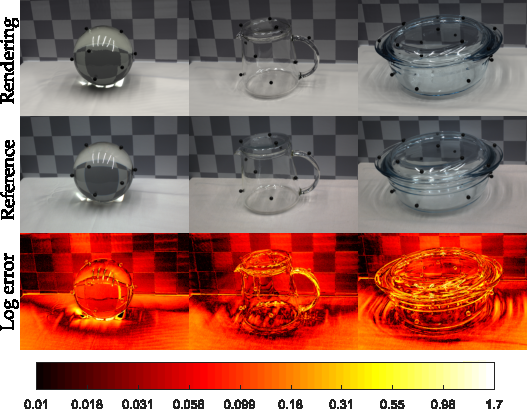
\includegraphics[height=4.3cm]{figures/comparison} & \hspace{2em}
	 \includegraphics[height=4.3cm]{figures/glass_bowl_analysis_by_synthesis}  \\
\end{tabular}
\caption{To the left, comparing quantitatively renderings (top row) with real images (mid row). Error is shown in the bottom row. On the right, estimating the absorption parameter $\sigma_a$ for the glass bowl. Each coefficient was estimated independently. Each dot in the graph corresponds to a rendered image. }
\label{fig:glasscomparison}
\end{figure}
The role of our proof of concept in Contribution~\ref{sec:juice} is dual. First, it tells us that it is important to validate renderings with photographs, to ensure that the rendering matches the appearance in the real world. Secondly, it tells us that this comparison has to be achieved fast, so that multiple parameters can be tested, or even estimated, depending on the application. We will discuss the first aspect in the rest of this section, referring to the next section for a more complete discussion on fast rendering of scattering materials. In our main contribution~\ref{sec:glass}, we strive to improve upon the previous results of comparing rendering with images, for a different application. In this case, we are comparing images of glass objects. As it is true for scattering materials, the appearance of glass objects is greatly influenced by the surrounding scene, making the scene estimation even more important for this application. We use a full pipeline to accurately estimate the scene, scan glass objects with CT scanners and place them in the scene for final rendering. Our main contribution of this work is actually the pipeline, that allows researchers to compare pictures and renderings of glass objects, getting a quantitative comparison at the end. This allows researchers to experiment with each step of the pipeline, improving upon the state of the art techniques used. As we can see from Figure~\ref{fig:glasscomparison} on the left, we are able to quantitatively compare images of glass objects with pictures, something that as never been done before. This ability of qualitatively compare images and rendering would allow in the future to further improve existing techniques in acquisition, rendering and reconstruction. Given our improved reconstruction results, we can estimate material properties much more accurately than our previous contribution. In this particular case, we measure both the relative index of refraction $\eta$ and the spectral absorption coefficient $\sigma_a$ for each of the glass objects, as we can see in Figure~\ref{fig:glasscomparison} to the right. Note that each point of the graph is a rendering, so it becomes essential to generate a great number of images to estimate the material properties. Since we want accuracy, we need to use unbiased path tracing, that we accelerate using the GPU and execute at lower resolutions to achieve fast and accurate rendering of these images. 

\section{Interactive rendering of scattering media}
\begin{figure}[t]
\centering
\begin{tabular}{@{}c@{$\,$}c@{}c@{}c@{}}
& directional dipole, 6 fps & standard dipole and VPLs \\
\begin{sideways}\hspace*{1.5em}our method\end{sideways} &
\includegraphics[width=0.43\columnwidth]{figures/candle_holder_directional_6fps.png} &
\includegraphics[width=0.43\columnwidth]{figures/candle_holder_jensen_converged.png} \\[-4pt]
\begin{sideways}\hspace*{1.7em}ray tracer\end{sideways} &
\includegraphics[width=0.43\columnwidth]{figures/scene_comparison_optix_6fps.png} &
\includegraphics[width=0.43\columnwidth]{figures/scene_comparison_converged.png} \\[-0.5ex]
& directional dipole, 6 fps & directional dipole, reference \\[-1ex]
\end{tabular}
\caption{Equal time comparison (left column) of our method with the reference method and qualitative comparison with diffuse subsurface scattering (upper right) and the converged reference solution (lower right). The scene is lit by a point light in a white grapefruit candle holder.} % Emerging light illuminates a diffuse Stanford Bunny on a tabletop.}
\label{fig:optixcomparison}
\end{figure}

After discussing photorealistic rendering in the previous section, in this section we start discussing our first technique that brings photorealistic rendering into the interactive domain. We also here take inspiration from Contribution~\ref{sec:juice}: in the previous section, we discussed the importance of physically based material. In this section, we present an example that allows us to achieve a better photorealistic look.

Our Contribution~\ref{sec:interactivedirsss} is a rasterization-based caching scheme to improve efficiency of existing techniques. The most important contribution in this technique is that allows rendering using \emph{directional} BSSRDFs like the directional dipole discussed in Section~\ref{sec:analyticalbssrdf}. Our technique allows to render with any BSSRDF analytical model that depends on $\vec{\omega}_i$, the direction of the incoming light. This allows more subtle scattering effects to be computed, accounting partially for single scattering, that in previous techniques needed to be added separately. See Figure~\ref{fig:optixcomparison}, top row, for a comparison between the standard dipole~\cite{Jensen2001} and the directional dipole~\cite{Frisvad2014}. Most of the interactive and real time techniques for rendering BSSRDFs assume that the BSSRDF is function of the distance between the point of incidence and emergence only. This can be exploited for different optimizations, like filtering, precomputation or tabulation, that are not feasible anymore when it comes to using a directional technique. Our technique is unique in handling this specific type of directional dipoles in the interactive domain. 

In the classification of different techniques presented in Chapter~\ref{sec:related}, our technique is mostly a caching technique, with some filtering required to assemble the final image. Our technique leverages the strengths of rasterization, storing progressive maps of scattered radiosity rendered from different directions around the object. We can now account for the directionality of the light in the computation, and in addition progressively store the intermediate result as soon as the light and the object do not change. We contribute with a fully interactive technique, that does not require neither precomputation nor texture parameterization. Given this features, we can apply this technique to procedural deformable objects, something that is generally quite difficult to achieve with precomputation techniques. In our technique, we contribute with an improved sampling scheme, that via our maps can sample radiosity always close to the light source, allowing light to propagate through objects and around sharp corners. This can be seen in particular in Figure~\ref{fig:optixcomparison}, in the top left image, where a point light source is places inside a candleholder made of a scattering material.  

As another contribution of our technique, we leverage our scattered radiosity maps to place VPLs on the surface of the objects. This allows to transfer emergent light onto other surfaces. An example can be seen in Figure~\ref{fig:optixcomparison}, where we transport the light from a point light inside an object on the outside, illuminating the bunny on the tabletop. In the same figure, we can see on how we successfully compare to a fully path traced simulation (bottom right) that in the same time we render our solution cannot achieve the same results, looking unconverged and noisy (bottom left).

To sum up, the take away home message of this technique is that improved physical models, such as the directional dipole, sometimes do not allow us to reuse previous work. So, we need to develop new techniques to achieve interactive result, so that we can include these more accurate effects. Moreover, the benefits of caching data in this case become particularly apparent, since they allow us to recycle the stored radiosity for another technique to use. 

\section{Interactive stable ray tracing}

\begin{figure}[t]
\begin{tabular}{@{}c@{}c@{}@{}c@{}}
	 \includegraphics[width=0.32\textwidth]{figures/ss_2x_rect_370_300_300_300_frame_211.png} &
		 \includegraphics[width=0.32\textwidth]{figures/ss_2x_taa_rect_370_300_300_300_frame_211.png} &
		  \includegraphics[width=0.32\textwidth]{figures/ss_32x_rect_370_300_300_300_frame_211.png} \\	 
Supersampling, 2 spp & Supersampling, 2 spp 	& Supersampling, 32 spp \\
  					 & + temporal antialiasing 	&  \\
sharpness: 0.7924 & sharpness: 0.5348 & sharpness: 0.6771  \\
	 \includegraphics[width=0.32\textwidth]{figures/srt_1_rect_370_300_300_300_frame_211.png} &
	 	 \includegraphics[width=0.32\textwidth]{figures/srt_1_ti_rect_370_300_300_300_frame_211.png} &
	  \includegraphics[width=0.32\textwidth]{figures/ss_32x_rect_370_300_300_300_frame_211.png}
 \\
Stable RT, 1 spp & Stable RT, 1 spp & Supersampling, 32 spp \\
 & + temporal integration &  \\
sharpness: 0.7085 & sharpness: 0.6060 & sharpness: 0.6771 \\[-1.5ex]
\end{tabular}
\caption{Different techniques applied to a frame in the Sponza video, equal time comparison. Sharpness is also shown (higher is sharper). Stable ray tracing offers a less noisy result (first column) compared to reference (third column). When temporal techniques are applied (second column) Stable ray tracing yields the sharper result.  }
\label{fig:sponza_video_frame}
\end{figure}
After dealing with subsurface scattering, we continue exploring the spectrum of interactive photorealistic techniques in Contribution~\ref{sec:srt}. As in the previous section, we use caching as a technique to improve existing physically based techniques. In this contribution, in particular, we discuss the problem of achieving renderings that are temporally stable. In our case, we discuss a possible solution applicable to interactive ray tracing.  

When going to a interactive or real time ray tracing technique, the number of paths we can shoot per pixel becomes extremely limited, in the order or one or two. Also, the shading locations change every frame, causing a noisy image, both spatially and temporally. Existing techniques, namely temporal anti aliasing, can mitigate the problem, tough they generally introduce blur. in our technique, we recycle shading locations across frames. Shading always the same points, we improve temporal stability, while retaining sharpness. We can see the results in Figure~\ref{fig:sponza_video_frame}. In the result we can see how stable ray tracing yields a  sharper result than temporal antialiasing. The technique contributes as a rendering system to improve temporal stability: other existing techniques can be further applies on top to further improve shading quality. 

Another contribution of this technique is that it shows how we can leverage the strength of one interactive technique, namely ray tracing, against the most commonly used rasterization. Current hardware does not allow shading locations to be arbitrarily chosen within a pixel, relying on fixed patterns (such as in MSAA). In our technique, we allow shading locations to vary in screen space per pixel, while staying the same in world space. 

Finally, another advantage of this technique, in particular in a photorealistic rendering context, is that it allows to store shading information across frames, e.g. to store indirect illumination. This will allow in the future to extend the technique with other sort of data, to further improve the technique. This gives the take home message of this technique: we need generic, robust techniques that can be applied in a variety of situations, inexpensive and that can work together with existing techniques. We believe that stable ray tracing satisfies these characteristics. 

\section{Applying interactive photorealistic techniques}
\begin{figure}[t]
\centering
\begin{tabular}{@{}c@{}c@{}}
	 \includegraphics[height = 4.3cm]{figures/screen1_crop} &
		 \includegraphics[height = 4.3cm]{figures/person} \\[-2.5ex]
\end{tabular}
  \caption{Pictures illustrating our VR demo application, with an in-game screenshot (left) and a picture of the setup (right). }
  \label{fig:vrbrdfimage}
\end{figure}
In contribution~\ref{sec:vrbrdf}, we push physically based rendering even further, applying it to virtual reality. In this context, applications need to consistently perform at 90 frames per second or faster, to avoid issues for the users, e.g. dizziness or motion sickness. In our application, we modify the rendering pipeline of the Unity game engine  to include physically based BRDFs, in the discretized form of the MERL database, as described in Section~\ref{sec:empiricalbrdf}. This proof of concept was born as an inspecting tool to debug physically based materials, aided by the provided in game controllers (see Figure~\ref{fig:vrbrdfimage}). The application gives us a glimpse on how photorealistic materials are able to augment the immersiveness of the application, which is paramount in virtual reality applications.

\section{Discussion}
In the previous sections, we showed how our contribution overall contribute to the goal of expanding interactive technique towards a more physically accurate framework. The natural step of the topics discussed in this thesis is to further expand the techniques in photorealism, by including as an example more accurate physical models, but retaining the same performance level. In the following, we discuss some possible avenues of expansion of our work.

\textbf{Validating path tracing}. Some avenues are possible in continuing the work we initiated in Contributions~\ref{sec:juice} and \ref{sec:glass}. In particular, we would like to continue our initial goal of validating path tracing. This would require expanding the technique to be more accurate, in particular in regards to geometry. For a more complete validation, we would like to expand the technique to handle fully scattering materials instead of glass only. Other avenues of research are possible in regards of estimating parameters: scattering parameters ($\sigma_a$, $\sigma_s$ and $g$) are obvious candidates for a further expansion.

\textbf{Hybrid rasterization-ray tracing rendering techniques}. As for now, we focused on our technique to be exclusively rasterization or ray tracing based. Some potential improvements can be thought by combining the two techniques. For example, some could think of an extension of our stable ray tracing in Contribution~\ref{sec:srt} to support our technique from Contribution~\ref{sec:interactivedirsss}. In this particular case, the scattered radiosity maps can be replaced by the stable ray traced points. The rasterization of the light G-buffer would still have to be executed, making this an hybrid technique.  Another example, in our virtual reality contribution~\ref{sec:vrbrdf}, would be to evaluate reflections via ray tracing, to properly include the overall contribution instead of an approximation via a precomputed probe.

\textbf{Virtual reality}. In recent year, virtual reality has become more prominent in real time applications. Given the hard constraints of virtual reality, the techniques we developed would need to be adapted to fit a virtual reality environment. In particular our stable ray tracing algorithm in Contribution~\ref{sec:srt} seems like a good fit for a virtual reality environment, that is particularly plagued by temporal stability issues. 

\textbf{Dataset generation for machine learning}. Interactive techniques for photorealistic rendering allow generating image data much faster than traditional techniques. This makes them particularly useful to generate synthetic data to train image based machine learning techniques.                                    %Chapter 1
\chapter{Conclusions}

\begin{itemize}
\item Investigated the challenges in comparing images with photorealistic renderings (Contributions~\ref{sec:glass}, \ref{sec:juice}).
\item Proposed a reconstruction and assembly pipeline that allows to compare images to renderings of the same scene (Contribution~\ref{sec:glass}).
\item Created a new dataset of transparent objects scene and CT scan data (Contribution~\ref{sec:glass}).
\item Proposed new techniques to estimate material parameters (Contributions~\ref{sec:glass}, \ref{sec:juice}).
\item Explored the challenges of fast interactive photorealistic rendering for rendering and quality assurance (Contributions~\ref{sec:juice},\ref{sec:interactivedirsss}).
\item Demonstrated the first interactive application of light-directional subsurface scattering (Contribution~\ref{sec:interactivedirsss}).
\item Developed a new interactive ray tracing technique to improve temporal stability without sacrificing sharpness (Contribution~\ref{sec:srt}).
\item Created new interactive rendering technques on to improve photorealistic light transport (Contributions~\ref{sec:interactivedirsss}, \ref{sec:srt}).
\item Created a novel Virtual Reality application to showcase phisically based materials in a hard real time context (Contribution~\ref{sec:vrbrdf}).
\end{itemize}                                  %Chapter 1
\appendix
\renewcommand{\thechapter}{\Roman{chapter}}
\chapter{Scene reassembly after multimodal digitization and pipeline evaluation using photorealistic rendering}
\includepdf[pages={-}]{papers/ao-56-27-7679.pdf}

\chapter{Interactive Appearance Prediction for Cloudy Beverages}
\includepdf[pages={-}]{papers/juice_mam16_submitted.pdf}

\chapter{Interactive Directional Subsurface Scattering and Transport of Emergent Light}
\includepdf[pages={-}]{papers/dirsssgpu_visual_computing.pdf}

\chapter{Interactive Stable Ray Tracing}
\includepdf[pages={-}]{papers/stable_rt_final.pdf}

\chapter{Virtual Reality inspection and painting with measured BRDFs}
\includepdf[pages={-}]{papers/abstract.pdf}

\chapter{Note on measuring BSSRDFs}
\includepdf[pages={-}]{papers/bssrdf_note.pdf}

\chapter{Note on efficient color calibration on the GLASS project}
\includepdf[pages={-}]{papers/color_calibration_note.pdf}

\chapter{Note clarifying BSSRDF importance sampling by Mertens et al.}
\includepdf[pages={-}]{papers/mertens_note.pdf}

\chapter{VirtualTable: a projection augmented reality game}
\includepdf[pages={-}]{papers/poster_siggraph.pdf}

\chapter{Our 3D Vision Data-Sets in the Making}
\includepdf[pages={2-}]{papers/robds.pdf}

                                 %Appendix A
%-----------
% Backmatter
%-----------
\backmatter
\chaptermark{Bibliography}
\renewcommand{\sectionmark}[1]{\markright{#1}}
\sectionmark{Bibliography}
\addcontentsline{toc}{chapter}{Bibliography}        %Force addition of Bibliography to TOC
\bibliographystyle{alpha}                           %Use alpha codes for references
\bibliography{references}                           %Bibliography file called
\end{document}
% % % EOF % % %